\section{Empirical results}
Malapert uses benchmark data by Daste. For design purposes, I created my own set of randomized job lists, with $s_j, p_j \in [1, 20]$ and $d_j \in [1, 10n]$ where $n$ is the number of jobs. Here is the Python code used:

\lstset{language=Python}
\begin{lstlisting}
import random

random.seed(None)

for i in range(11, 20) + range(10,100,10):
    for j in range(1, 10):
        with open( "data_" + str(i) + "_" + str(j), "wb") as csvfile:
            csvwriter = csv.writer(csvfile, delimiter=",")
            csvwriter.writerow(['s_j', 'p_j', 'd_j'])
            for job in range(i):
                csvwriter.writerow([random.randrange(1,20), random.randrange(1,20), random.randrange(1,5*i)])
        csvfile.close()
\end{lstlisting}

CSV files can be read in with \texttt{IloCsvReader} and \texttt{IloCsvLine}.

\subsection{Comparison of CPU time used by various models}
Figure \ref{fig:comp_times} shows the CPU time used by the models. Ten sample
job sets are used per number of jobs, represented as $\left[\{10.0, \dots, 10.9\},
\{11.0, \dots, 11.9\},\dots \right]$ on the horizontal axis. The models were run
on an i7 Q740 CPU, which has $2 \times 4$ cores. Cplex supports multithreading
and as such, elapsed wall clock time is significantly lower in most cases.
\begin{figure}
\centering

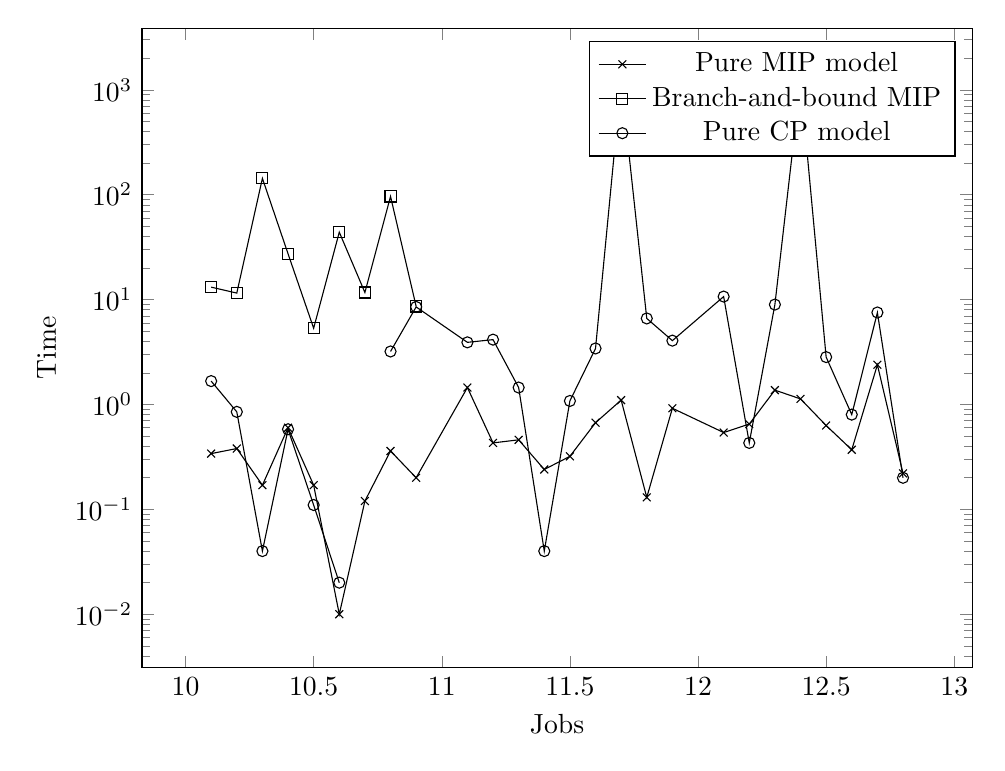
\begin{tikzpicture}
  \begin{semilogyaxis}[xlabel=Jobs, ylabel=Time, width=\textwidth,
  height=0.8\textwidth]
  \addplot[color=black, mark=x ] coordinates { % MIP model times
(10.1, 0.34)
(10.2, 0.38)
(10.3, 0.17)
(10.4, 0.6)
(10.5, 0.17)
(10.6, 0.01)
(10.7, 0.12)
(10.8, 0.36)
(10.9, 0.2)
(11.1, 1.45)
(11.2, 0.43)
(11.3, 0.46)
(11.4, 0.24)
(11.5, 0.32)
(11.6, 0.67)
(11.7, 1.1)
(11.8, 0.13)
(11.9, 0.92)
(12.1, 0.54)
(12.2, 0.65)
(12.3, 1.37)
(12.4, 1.13)
(12.5, 0.63)
(12.6, 0.37)
(12.7, 2.39)
(12.8, 0.22)
  };
  \addlegendentry{Pure MIP model}
  \addplot[color=black, mark=square] coordinates {
(10.1, 13.14)
(10.2, 11.53)
(10.3, 143.11)
(10.4, 27.34)
(10.5, 5.33)
(10.6, 43.9)
(10.7, 11.68)
(10.8, 96.27)
(10.9, 8.6)
  };
  \addlegendentry{Branch-and-bound MIP}
  \addplot[color=black, mark=o] coordinates {
(10.1, 1.67)
(10.2, 0.85)
(10.3, 0.04)
(10.4, 0.58)
(10.5, 0.11)
(10.6, 0.02)

(10.8, 3.2)
(10.9, 8.51)
(11.1, 3.91)
(11.2, 4.15)
(11.3, 1.45)
(11.4, 0.04)
(11.5, 1.08)
(11.6, 3.42)
(11.7, 1200)
(11.8, 6.61)
(11.9, 4.06)
(12.1, 10.68)
(12.2, 0.43)
(12.3, 8.96)
(12.4, 1200)
(12.5, 2.83)
(12.6, 0.8)
(12.7, 7.53)
(12.8, 0.2)
};
  \addlegendentry{Pure CP model}
  \end{semilogyaxis}
\end{tikzpicture}

\caption{Comparison of CPU time used by different models.}
\label{fig:comp_times}
\end{figure}



